\documentclass[a4paper,10pt]{article}
\usepackage[utf8]{inputenc}
\usepackage{lmodern}
\usepackage[T1]{fontenc}
\usepackage[italian]{babel}
\usepackage{graphicx}
\usepackage{listings}
\usepackage{color}
\usepackage{geometry}
\geometry{a4paper, left=1.5cm, right=1.5cm, top=2cm, bottom=1.5cm}
\definecolor{lightgray}{gray}{0.9}
\setlength{\parindent}{5mm}
\linespread{1}

 

\begin{document}
	
	\title{Programmazione ad Oggetti\\Relazione progetto Kalk}
	\author{Mihai Eni\\Matricola 1101684}
	\date{08-09-2018}
    \maketitle
        \begin{figure}[!h]
            \begin{center}
                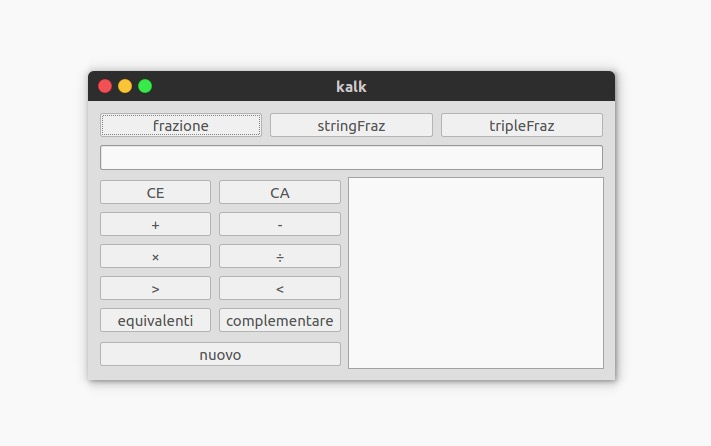
\includegraphics[scale=0.5]{img/kalk.jpeg}
                \caption{Schermata di default Kalk}
            \end{center}
        \end{figure}    
    
    \newpage
	\tableofcontents
	\newpage
	
    \section{Scopo del Progetto}
    La richiesta del progetto è la realizzazione di una calcolatrice che opera con diversi titpi di dato
    I dati disponibili nella calcolatrice sono i seguenti : 
        \begin{itemize}
            \item \textbf{frazione}, sono frazioni dove numeratore e denominatore sono numeri reali, permettono di eseguire le principali operazioni algebriche e di confronto tra frazioni;
            \item \textbf{stringFraz}, sono frazioni con l'aggiunta di \textit{mid } un parametro stringa, questo tipo di frazioni peremettono le stesse operazioni di \textit{frazione};
            \item \textbf{tripleFraz}, sono frazioni con l'aggiunta di \textit{triple} un numero intero, anche quest'ultimoe peremettono le stesse operazioni di \textit{frazione};
        \end{itemize}
    La calcolatrice non cambia graficamente tra i tre tipi di dato,cambia l'implementazione.

	\section{Gerarchie utilizzate}
    \subsection{Gerarchia dei tipi di dato}
    \subsubsection{Classe Frazione}
        La classe Frazione rappresenta la divisione tra numeri reali mediante frazioni. Ha due campi dato di tipo intero che indetificano numeratore e denominatore. 
        \\Esegue l'overloading virtuale di diversi metodi:
        \begin{itemize}
            \item \textbf{virtual frazione*  operator +(const frazione*  ) const;}: restituisce un puntatore ad una frazione uguale alla somma tra 2 frazioni;
            \item \textbf{virtual frazione*  operator -(const frazione*  ) const;}: restituisce un puntatore ad una frazione uguale alla differenza tra 2 frazioni;
            \item \textbf{virtual fr
            azione*  operator*(const frazione*  ) const;}: restituisce un puntatore ad una frazione uguale alla moltiplicazione tra 2 frazioni;
            \item \textbf{virtual frazione*  operator/(const frazione*  ) const;}: restitutisce un puntatore ad una frazione uguale alla divisione tra 2 frazioni;
            \item \textbf{virtual bool operator==(const frazione*  ) const;}: restituisce un booleano che indica se le frazioni sono uguali;
            \item \textbf{virtual bool operator!=(const frazione*  ) const;} restituisce un booleano che indica se le frazioni sono diverse;
            \item \textbf{virtual bool operator<(const frazione*  ) const;}: restituisce un booleano che indica se una frazione è minore dell'altra;
            \item \textbf{virtual bool operator>(const frazione*  ) const;}: restituisce un booleano che indica se una frazione è maggiore dell'altra.
        \end{itemize}
        Definisce i seguenti metodi virtuali:
        \begin{itemize}
            \item \textbf{virtual frazione* clone() const;}: restituisce un puntatore alla copia della frazione;
            \item \textbf{virtual std::string toString()const;}: restituisce una \textit{std::string} che rappresenta la frazione;
            \item \textbf{virtual int getMCD() const;}: restiruisce il massimo comun divisore tra numeratore e denominatore;
            \item \textbf{virtual void reduce();}: riduce ai minimi termini la frazione;
            \item \textbf{virtual frazione*  minima() const;}: restituisce un puntatore alla copia della frazione ridotta ai minimi termine;
            \item \textbf{virtual double razionale() const;}: ritorna il razionale corrispondente alla frazione;
            \item \textbf{virtual frazione*  complementare() const;} ritorna un puntatore alla frazione complementare.
        \end{itemize}
    \subsubsection{Classe stringFraz}
        La classe \textit{stringFraz}, derivata dalla classe \textit{frazione}, rappresenta un tipo di frazione alla quale è stata aggiunta una stringa centrale.
       \\ Esegue l'override dei seguenti metodi virtuali della classe frazione:
        \begin{itemize}
            \item \textbf{stringFraz* clone() const;}
            \item \textbf{stringFraz* minima() const;}
            \item \textbf{stringFraz* complementare() const;}
            \item \textbf{stringFraz* operator +(const frazione* ) const override;}
            \item \textbf{stringFraz* operator -(const frazione* ) const override;}
            \item \textbf{stringFraz* operator *(const frazione* ) const override;}
            \item \textbf{stringFraz* operator /(const frazione* ) const override;}
            \item \textbf{bool operator==(const frazione* ) const override;}
            \item \textbf{bool operator!=(const frazione* ) const override;}
            \item \textbf{bool operator<(const frazione* ) const override;}
            \item \textbf{bool operator>(const frazione* ) const override;}
        \end{itemize}
    \subsubsection{Classe tripleFraz}
        La classe \textit{tripleFraz}, derivata dalla classe \textit{frazione}, rappresenta una doppia frazione mediante l'aggiunta di un intero chaimato \textbf{triple}. Triple viene visto come un secondo numeratore di conseguenza si vengono a creare 2 frazioni con lo stesso denominatore e 2 numeratori che possono essere  uguali.
        \\Esegue l'override dei seguenti metodi virtuali della classe frazione:
        \begin{itemize}
            \item \textbf{tripleFraz* clone() const;}
            \item \textbf{int getMCD() const;}
            \item \textbf{void reduce();}
            \item \textbf{tripleFraz* minima() const;}
            \item \textbf{double razionale() const;}
            \item \textbf{tripleFraz* complementare() const;}
            \item \textbf{tripleFraz* operator +(const frazione* ) const;}
            \item \textbf{tripleFraz* operator -(const frazione* ) const;}
            \item \textbf{tripleFraz* operator*(const frazione* ) const;}
            \item \textbf{tripleFraz* operator/(const frazione* ) const;}
            \item \textbf{bool operator==(const frazione* ) const;}
            \item \textbf{bool operator!=(const frazione* ) const;}
            \item \textbf{bool operator<(const frazione* ) const;}
            \item \textbf{bool operator>(const frazione* ) const;}
        \end{itemize}
    \newpage
    \subsection{Gerarchia del controllo input}
        La gerarchia del controllo input serve per controllare che l'input sia conforme  per la successiva creazione dei tipi di dato. Il controllo input è formato da una classe base astratta \textbf{check}, da cui derivano tutte le classi concrete del controllo input come \textbf{checkFraz}, \textbf{checkString} e \textbf{checkTriple}
    \subsubsection{Classe check}
        La classe base  astratta \textit{check} serve per contenere il nome dei parametri da inserire nell'input
        \\Definisce i seguenti metodi propri:
        \begin{itemize}
            \item \textbf{std::list<QString> getParametri() const;}: serve a ottenere il nome dei parametri dei tipi di dato;
            \item \textbf{void addParemetro(const QString);}: serve contenere il valore di ciascun parametro definito nell'input;
        \end{itemize}
        Definisce i  seguenti metodi virtuali puri:
        \begin{itemize}
            \item \textbf{bool virtual parser(QString, QString$\&$) =0;}: serve per controllare che l'input inserito sia corretto rispetto al tipo di dato;
            \item \textbf{virtual frazione* getFrazione(std::vector<QString>*)const=0;}: usato per creare il tipo di dato con i valori inseriti nell'input; 
        \end{itemize}
    \subsubsection{Classe checkFraz}
        La classe \textit{checkFraz} derivata dalla classe astratta \textbf{check}: serve per definire il nome dei parametri e per il controllo del input del dato \textit{frazione}.
        \\Implenta i seguenti metodi:
        \begin{itemize}
            \item \textbf{bool virtual parser(QString, QString$\&$);} serve per controllare che l'input del numeratore e del denominatore sia un numero intero;
            \item \textbf{virtual frazione* getFrazione(std::vector<QString>*)const=0;}: usato per creare una frazione una volta che il parser è stato eseguito su tutti i parametri; 
        \end{itemize}
    \subsubsection{Classe checkString}
        La classe  \textit{checkString} derivata dalla classe astratta \textbf{check} serve per definire il nome dei parametri e per il controllo del input del dato \textit{stringFraz}.
        \\Implenta i seguenti metodi:
        \begin{itemize}
            \item \textbf{bool virtual parser(QString, QString$\&$);} serve a controllare che l'input per la stringa mid sia composto solo da lettere e numeri reali;
            \item \textbf{virtual frazione* getFrazione(std::vector<QString>*)const=0;}: usato per creare una stringFraz dopo che il parser è stato eseguito su tutti i parametri. 
        \end{itemize}
    \subsubsection{Classe checkTriple}
        La classe \textit{checkString} derivata dalla classe astratta \textbf{check} serve a definire il nome dei parametri e per il controllo del input del dato \textit{tripleFraz}.
        \\Implenta i seguenti metodi:
        \begin{itemize}
            \item \textbf{bool virtual parser(QString, QString$\&$);} usato per controllare che l'input per triple sia un numero reale;
            \item \textbf{virtual frazione* getFrazione(std::vector<QString>*)const=0;}: usato per creare una stringFraz dopo che il parser è stato eseguito su tutti i parametri.
        \end{itemize}
    \newpage
    \section{Classe contenitore Kalk}
        La classe \textit{Kalk} è la classe contenitore generale che viene usata per mettere in communicazione i tre tipi di oggetti che contiene al suo interno:
        \begin{itemize}
            \item \textbf{model}: gestore delle checkS;
            \item \textbf{input}: una vista per l'input;
            \item \textbf{view}: la vista della calcolatrice.
        \end{itemize}
    \subsection{Classe model}
        La classe \textit{model} permette lo scambio del tipo di dato tra \textit{frazione}, \textit{stringFraz} e \textit{tripleFraz} a livello logico e gestisce le operazioni dei vari tipi di dato. Contiene al suo interno i \textit{check} per fare l'input, tutte le frazioni che vengono create, 2 operandi per fare le operazioni tra frazioni, result che serve  salvare il risultato delle oprazioni e i valori inseriti nell'input.
        Contiene i seguenti SLOT:
        \begin{itemize}
        \item \textbf{void setOperand(QListWidgetItem*);}: usato per assegnare agli operandi le frazioni immagazzinate;
        \item \textbf{void changeCheck(int);}: serve a cambiare il tipo di \textit{check} e conseguenza tipo di dato usato;
        \item \textbf{void openInput();} usato per comunicare a \textbf{kalk} di aprire l'input;
        \item \textbf{void getNewValore(QString, QString);} uasato per immagazzinare l'utimo input inserito.
        \end{itemize}
        Contiene i seguenti SIGNALS:
        \begin{itemize}
            \item \textbf{void sendInputKo(QString);}: per communicare a \textbf{kalk} che l'input è errato;
            \item \textbf{void sendCloseInput();}: per communicare a \textbf{kalk} che l'input è corretto e quindi chiudere l'input;
            \item \textbf{void sendToVideo(QString);}: per mandare alla \textbf{view} una stringa da mettere a video;
            \item \textbf{void sendChangedCheck();}: comunica a \textbf{kalk} che il cambio della \textit{check} è avvenuto correttamente.
        \end{itemize}
    \subsection{Classe input}
        La classe \textit{input} serve per poter inserire l'input e inviarlo al model. Contiene una \textit{QLineEdit()} usata per inserire l'input e una \textit{QLabel()} usata per comunicare quale parametro inserire;
    \subsection{Calsse view}
        La classe \textit{view} serve per formare la GUI e contiene:
        \begin{itemize}
            \item \textbf{QLineEdit* constVideo;}: serve per fare vedere l'operatore selezionato, il risultato oppure l'errore avenuto all'iterno di un'operazione;
            \item \textbf{QListWidget* oggetti;}: serve per far vedere tutte le frazioni create e salvare i risultati;
            \item \textbf{QVBoxLayout* vista;}: layout generale usato per contenere \textit{constVideo} ,\textit{text} e tutti i pulsanti delle operazioni.
        \end{itemize}
        Contiene i seguenti SLOT:
        \begin{itemize}
            \item \textbf{void addToVideo(QString);} serve per cambiare il contenuto di \textit{constVideo};
            \item \textbf{void refreshFrazioni(std::vector<QString>);} serve per aggiornare il contenuto di \textit{oggetti}.
        \end{itemize}
        Contiene i seguenti SIGNALS che vengono inviati quando si preme un pulsante nella tastiera e quindi indica l'operazione da fare:
        \begin{itemize}
            \item \textit{void sendChangeCheck(int);}
            \item \textit{void sendSelectOperand(QListWidgetItem*);}
            \item \textit{void sendOpenInput();}
            \item \textit{void sendSomma();}
            \item \textit{void sendSottrazione();}
            \item \textit{void sendMoltiplicazione();}
            \item \textit{void sendDivisione();}
            \item \textit{void sendMaggiore();}
            \item \textit{void sendMinore();}
            \item \textit{void sendUgualianza();}
            \item \textit{void sendComplementare();}
            \item \textit{void sendClearElement();}
            \item \textit{void sendClearAll();}
            \item \textit{void sendCloseInput();}
        \end{itemize}
\newpage
        \section{Descrizione del codice polimorfo}
        Nelle classi precedentemente descritte sono presenti metodi che eseguono chiamate polimorfe.
        Per fare esempi di chiamate polimorfe ogni chiamata fatta dalla classe \textit{model} sugli operandi, il tipo statico del puntatore è di tipo \textit{frazione*} mentre l'oggetto puntato potrebbe essere di tipo \textit{frazione},\textit{stringFraz} o \textit{tripleFraz}.
        Altri esempi di chiamate polimorfe possono essere individuati nella classe \textit{check} nelle operazioni di input, dopo vengono chiamati i metodi \textit{parser} ed altri.

        \section{Manuale utente}
        \subsection{Avvio}
        All’avvio dell’applicazione Kalk questa si troverà nella scheda \textit{Frazione}, per gli altri tipi di dato basterà premere i tasti in alto a destra cambiando così tipo di dato su cui operare.
        \subsection{Struttura}
        La calcolatrice è divisa in tre aree principali:
        \begin{itemize}
            \item nell’area sulla destra è presente una lista che in base al tipo di dato su cui si sta lavorando mostra tutti gli oggetti creati fino a quel momento per il tipo di dato corrente;
            \item la seconda parte sotto i tipi di dato è la visualizazione dei dati inseriti, dei risultati e degli erorri sulle operazioni;
            \item e una terza contenete tutti i pulsanti delle operazioni disponibili.
        \end{itemize}  
        \subsection{Dinamica operazioni}
        La dinamica di selezione di operandi e operazioni è leggermente diversa dalla normale calcolatrice:
        \begin{itemize}
            \item per fare una operazioni selzionare prima gli operandi sulla destra e premere poi il pulsante con l'operazione;
            \item per inserire un nuovo dato premere nuovo e poi si aprira l'input dove ci sono i nomi dei parametri e la barra dove inserire il valore del paramentro
        \end{itemize}
        \section{Ore utilizzate}
        Sono state utilizzate le seguenti ore alla consegna:
        \begin{itemize}
            \item \textbf{Progettazione}: 2 ore;
            \item \textbf{Studio delle librerie di QT}: 20 ore;
            \item \textbf{Scrittura codice}: 23 ore;
            \item \textbf{Scrittura relazione}: 2 ore;
            \item \textbf{Test}: 1 ora;
            \item \textbf{Traduzione gerarchia tipi in Java}: 2 ore.
        \end{itemize}
        \section{Ambiente di sviluppo}
        \begin{itemize}
            \item Sistema operativo: 16.04 LTS
            \item gcc version 5.4.0 20160609
            \item Qt version 5.5.1
            \item QMake version 3.0
        \end{itemize}
\end{document}\grid
\grid
